% a-project.tex, v-1.0.3 marcoreis baseado no
% abntex2-modelo-trabalho-academico.tex, v-1.9.7 laurocesar
% Copyright 2012-2018 by abnTeX2 group at http://www.abntex.net.br/ 
% 
% This work consists of the files ........
% 
% -----------------------------------------------------------------------------
% Modelo para desenvolvimento de documentação de projetos acadêmicos
% (tese de doutorado, dissertação de mestrado e trabalhos de monografias em geral) 
% em conformidade com ABNT NBR 14724:2011: Informação e documentação. 
% -----------------------------------------------------------------------------
% Opções para a documentação
%
% Fancy page headings 
%\documentclass[fancyheadings, subook]{Classes/a-prj}
%\documentclass[fancyheadings, sureport]{Classes/a-prj}
%
% Fancy chapters and sections headings 
%\documentclass[fancychapter, subook]{Classes/a-prj}
%\documentclass[fancychapter, sureport]{Classes/a-prj}
%
% Fancy page , chapters and sections headings
%\documentclass[fancyheadings, fancychapter, subook]{Classes/a-prj}
\documentclass[fancyheadings, fancychapter, sureport]{Classes/a-report}
%
% -----------------------------------------------------------------------------
% Alguns comandos para a fancy page headings)
%
% Page header line width
%\footlinewidth{value}
%
% Page footer line width
%\headlinewidth{value}
%
% Page header and footer line width
%\headingslinewidth{value}
%
% Page header and footer lines without text
%\headingslinesonly
%
% The default line width is 0.3pt.
% Set the value to 0pt to remove the page header and/or footer line
%
% -------------------------------------------------------------------------------
% Formato de figuras suportado
% -------------------------------------------------------------------------------
% O formato das figuras depende da forma como o arquivo de saída é gerado.
% As figuras inseridas na pasta Figures serão automaticamente reconhecidas sem
% a necessidade de inserir a extensão do arquivo.
%
% O pdfLaTEX (PDF) suporta figuras com as extensões: pdf, jpg, png e mps.
%
% -------------------------------------------------------------------------------
% Árvore do diretório a-project.tex
%  Diretório
%       \Classes        (requerido)
%       \Figures        (requerido) --------------------------------->
%       \Figures\PDF    (optional)
%       \Figures\JPG    (optional) Figures located within these
%       \Figures\PNG    (optional) folders are searched automatically
%       \Figures\MPS    (optional)  by the a-prj class.
%       \Figures\EPS    (optional)
%       \Figures\PS     (optional) <--------------------------------
%       \Tables         (requerido)
%       \Others         (requerido)
%       \Chapters       (requerido)
%       \Appendices     (optional)
%       \References     (requerido)
%
% -------------------------------------------------------------------------------
% PDF File resumo
\ifpdf
    \hypersetup{
    	backref,
        colorlinks  = true,
        pdftitle    = Modelo de documentação,
        pdfauthor   = {Marco Reis, marco.a.reis@gmail.com},
        pdfsubject  = Mestre em Engenharia,
        pdfcreator  = Subtitulo,
        pdfproducer = PDFLatex,
        pdfkeywords = {documentação, latex, dissertação, tese}}

 \fi
%
% -------------------------------------------------------------------------------
% Relação de pacotes opcionais utilizados
\usepackage[utf8]{inputenc}
\usepackage[brazil]{babel}
\usepackage{longtable}
\usepackage{dcolumn}
\usepackage{multirow}
\usepackage{lscape}
%\usepackage{graphicx}
\usepackage{rotating}
%\usepackage{float,subfigure}
%\usepackage{graphicx, subfigure}
\usepackage{cite}
\usepackage[left=3cm,top=3cm,right=2cm,bottom=2cm]{geometry}
\usepackage[alf]{abntex2cite}
\usepackage{ifpdf}
\usepackage{shadow}
\usepackage{wrapfig}
\usepackage[normalem]{ulem}
\usepackage{makeidx}
\usepackage{yfonts}
\usepackage{algorithm}
\usepackage{algorithmic}
\usepackage{lmodern}
\usepackage[T1]{fontenc}
\usepackage{indentfirst}
\usepackage{color}
\usepackage{microtype}
\usepackage{lipsum}
\usepackage{caption}
\usepackage{subcaption}
\usepackage{plantuml}
\makeindex 
\setlength{\LTcapwidth}{\textwidth}
%
\newtheorem{theorem}{Teorema}
\newtheorem{definition}[theorem]{Definição}
%
% -------------------------------------------------------------------------------
% Configurações do pacote backref
\renewcommand{\backrefpagesname}{Citado na(s) página(s):~}
% Texto padrão antes do número das páginas
\renewcommand{\backref}{}
% Define os textos da citação
\renewcommand*{\backrefalt}[4]{
	\ifcase #1 %
		Nenhuma citação no texto.%
	\or
		Citado na página #2.%
	\else
		Citado #1 vezes nas páginas #2.%
	\fi
}
% 
% -------------------------------------------------------------------------------
% Início do documento raiz
\begin{document}
% Definição do título da página
    \university{Universidade Positivo}
	%\faculty{Programa de...}
	%\school{Escola de...}
% 
    %\course{Engenharia Elétrica}
    \typework{Relatório Final}
% 
	%\course{Mestrado em Modelagem Computacional e Tecnologia Industrial}
	%\typework{Disserta\c{c}\~ao de mestrado}
	%\typework{Exame de Qualificação de Mestrado}
% 
	%\course{Engenharia Elétrica}
	%\typework{Tese de doutorado}
	%\typework{Exame de Qualificação de doutorado}
%
% -------------------------------------------------------------------------------
% Informações gerais
    \thesistitle{Desenvolvimento de Site para Portfólio Fotográfico}
    \hidevolume
    \thesisvolume{Volume 1 of 1}
    \thesisauthor{Filipe Marques}
    \thesisauthorr{Guilherme Binhara }
    \thesisauthorrr{Gustavo Purkoot Ferreira }
    \thesisauthorrrr{Murilo Ribeiro}
    \thesisauthorrrrr{Vinicius de Assis}
    \thesisadvisor{Prof. Marco Reis, M.Eng.}
    %\hidecoadvisor
    %\thesiscoadvisor{Marco Reis}
    \thesismonthyear{Abril de 2025}
% 
    \maketitlepage
%
% ----------------------------------------------------------------------------
% Inserir Folha de rosto, Nota de estilo, folha de assinaturas, dedicatoria
    \begin{folharosto}

\begin{center}
\theauthor \\
\theauthorr \\
\theauthorrr \\
\theauthorrrr \\
\theauthorrrrr \\
%\theauthorrr \\
%\theauthorrrr \\
%\theauthorrrrr \\
\end{center}
\ \\
\ \\
\ \\
\ \\
\ \\
\begin{spacing}{2}
   \begin{center}
   {\LARGE {\bf \thetitle}}
   \end{center}
\end{spacing}
\ \\
\ \\
\ \\
\vspace*{85mm}
% \begin{flushright}

%    \begin{list}{}{
%       \setlength{\leftmargin}{7.5cm}
%       \setlength{\rightmargin}{0cm}
%       \setlength{\labelwidth}{0pt}
%       \setlength{\labelsep}{\leftmargin}}

%       \item \thetypework apresentada ao \thefaculty, Curso de \thecourse
%       do \theuniversity, como requisito parcial para a obten\c{c}\~ao do
%       t\'itulo de {\bf \thedegreetitle}.

%       \begin{list}{}{
%       \setlength{\leftmargin}{0cm}
%       \setlength{\rightmargin}{0cm}
%       \setlength{\labelwidth}{0pt}
%       \setlength{\labelsep}{\leftmargin}}

%       \item \'Area de conhecimento: Interdisciplinar

%       \item Orientador: \theadvisor
%       \newline \hspace*{2.1cm}  %{\it \theuniversity}

%       \end{list}
%    \end{list}

% \end{flushright}
\ \\
\ \\
\ \\
\ \\
%\begin{spacing}{1.5}
   \begin{center}
   Curitiba \par
   \theuniversity \par
   2025
   \end{center}
%\end{spacing}

\end{folharosto}

    %\begin{notaestilo}
Esta \thetypeworkthree foi elaborada considerando as normas de
estilo (i.e. est\'eticas e estruturais) propostas aprovadas pelo
colegiado do \thefacultytwo e est\~ao dispon\'iveis em formato
eletr\^onico ({\it download} na P\'agina Web
http:$//$ead.fieb.org.br$/$portal\_faculdades$/$dissertacoes-e-teses-mcti.html
ou solicita\c{c}\~ao via e-mail \`a secretaria do
programa) e em formato impresso somente para consulta. \\

Ressalta-se que o formato proposto considera diversos itens das
normas da Associa\c{c}\~ao Brasileira de Normas T\'ecnicas (ABNT),
entretanto opta-se, em alguns aspectos, seguir um estilo pr\'oprio
elaborado e amadurecido pelos professores do programa de
p\'os-gradua\c{c}\~ao supracitado.

\end{notaestilo}

    %\begin{folhaassinaturas}

%\thispagestyle{empty}

\def\signature#1#2{\parbox[b]{1in}{\smash{#1}\vskip12pt}
\hfill \parbox[t]{3in}{\shortstack{\vrule width 3in height
0.4pt\\\small#2}}}

\def\InstituicaoMembro#1#2{\parbox[b]{1in}{\smash{#1}\vskip12pt}
\hfill \parbox[t]{3in}{\shortstack{\vrule width 3in \\\small#2}}}

\def\signaturepage{%

    \begin{spacing}{1.5}
        \begin{center}
        {\LARGE \theuniversity} \\
        {\large \thefaculty} \\
        {\large \thecourse} \\
        \end{center}
    \end{spacing}

   \vskip 0.25in plus 0.4in minus 0.1in

    \begin{spacing}{1.5}
        \begin{sloppypar}
        A Banca Examinadora, constitu\'ida pelos professores abaixo
        listados, leram e recomendam a aprova\c{c}\~ao [com distin\c{c}\~ao] da
        \thetypeworktwo, intitulada ``\thetitle",
        apresentada no dia (dia) de (m\^es) de (ano), como requisito
        parcial para a obten\c{c}\~ao do t\'itulo de {\bf \thedegreetitle}.\\
        \end{sloppypar}
    \end{spacing}

    \def\sigskip{\vskip0.15in plus 0.2in minus 0.1in}
    \def\beginskip{\vskip0.3875in plus 0.2in minus 0.1in}

    \beginskip
    \signature{Orientador:}{Prof. Dr. \theadvisor} \\
    \InstituicaoMembro{}{\theuniversity} \\

    \sigskip
    \beginskip
    \signature{Membro externo da Banca:}{Prof. Dr. Nome completo} \\
    \InstituicaoMembro{}{Institui\c{c}\~ao do membro da banca} \\

    \sigskip
    \beginskip
    \signature{Membro externo da Banca:}{Prof. Dr. Nome completo} \\
    \InstituicaoMembro{}{Institui\c{c}\~ao do membro da banca} \\

    %\sigskip
    %\beginskip
   % \signature{Membro interno da Banca:}{Prof. Dr. Nome completo} \\
   % \InstituicaoMembro{}{Institui��o do membro da banca} \\

    \vfill
    \newpage
    \setcounter{page}{3}
}
%*********************************************************************


\signaturepage


\end{folhaassinaturas}

    %\include{Others/dedicatoria}
    %\include{Others/agradecimentos}
%

% ---------------------------------------------------------------------------
% Resumo/abstract, sumário e siglas
    \begin{romanpagenumbers}
        \begin{thesisresumo}
Este trabalho apresenta o desenvolvimento de um site institucional responsivo para portfólio fotográfico, com o objetivo de oferecer ao fotógrafo profissional Geovany uma plataforma leve e de fácil manutenção para exibir seus trabalhos e captar clientes. A pesquisa se insere no contexto do marketing digital para profissionais criativos, considerando a importância de uma presença online otimizada. O projeto foi realizado no contexto da disciplina de Análise e Projeto de Sistemas da Universidade Positivo, adota-se uma abordagem pragmática, baseada em metodologias ágeis (Scrum/Kanban) e boas práticas de UX/UI, aliada ao uso de ferramentas como Figma, Trello e GitHub. Foram realizados workshops de levantamento de requisitos, prototipação de interfaces e implementação do front-end em HTML5, CSS3 e JavaScript, com técnicas de otimização de desempenho. Contribui para o fortalecimento da visibilidade online de fotógrafos e para o aprendizado prático de gestão de projetos e desenvolvimento web.

\ \\

% use de três a cinco palavras-chave

\textbf{Palavras-chave}: Desenvolvimento Web, portfólio fotográfico, responsividade, metodologias ágeis, UX/UI

\end{thesisresumo}

        \begin{thesisabastract}
This work presents the development of a responsive institutional website for a photographic portfolio, aiming to provide professional photographer Geovany with a lightweight, easy-to-maintain platform to showcase his work and attract clients. The research is set within the context of the Analysis and Systems Design course at Universidade Positivo and adopts a pragmatic approach based on agile methodologies (Scrum/Kanban) and UX/UI best practices, supported by tools such as Figma, Trello, and GitHub. Requirements-gathering workshops, interface prototyping, and front-end implementation in HTML5, CSS3, and JavaScript were conducted, employing performance optimization techniques (image compression and lazy loading). As a contribution, this project strengthens photographers’ online visibility and offers practical learning in project management and web development.

\ \\

% use de tr�s a cinco palavras-chave

\textbf{Keywords}: web development; photographic portfolio; responsiveness; agile methodologies; UX/UI
\end{thesisabastract}


        % Make list of contents, tables and figures
        \thesiscontents
        
        %Include other required section
        %\begin{thesisabbreviations}
\begin{footnotesize}
\begin{longtable}[l]{p{2cm}l}
  tprax   \dotfill & \thefaculty \\
  WWW       \dotfill &  World Wide Web \\
\end{longtable}
\end{footnotesize}
\end{thesisabbreviations}

        %\begin{thesissymbols}
\begin{footnotesize}
\begin{longtable}[l]{p{2cm}l}
  $\partial$   \dotfill  & Bla bla bla \\
  $\prod$       \dotfill & ble ble ble \\
  $\partial$   \dotfill  & Bla bla bla \\
  $\prod$       \dotfill & ble ble ble \\
  $\partial$   \dotfill  & Bla bla bla \\
  $\prod$       \dotfill & ble ble ble \\
  $\partial$   \dotfill  & Bla bla bla \\
  $\prod$       \dotfill & ble ble ble \\
  $\partial$   \dotfill  & Bla bla bla \\
  $\prod$       \dotfill & ble ble ble \\
  $\partial$   \dotfill  & Bla bla bla \\
  $\prod$       \dotfill & ble ble ble \\
  $\partial$   \dotfill  & Bla bla bla \\
  $\prod$       \dotfill & ble ble ble \\
  $\partial$   \dotfill  & Bla bla bla \\
  $\prod$       \dotfill & ble ble ble \\
  $\partial$   \dotfill  & Bla bla bla \\
  $\prod$       \dotfill & ble ble ble \\
  $\partial$   \dotfill  & Bla bla bla \\
  $\prod$       \dotfill & ble ble ble \\
  $\partial$   \dotfill  & Bla bla bla \\
  $\prod$       \dotfill & ble ble ble \\
  $\partial$   \dotfill  & Bla bla bla \\
  $\prod$       \dotfill & ble ble ble \\
  $\partial$   \dotfill  & Bla bla bla \\
  $\prod$       \dotfill & ble ble ble \\
  $\partial$   \dotfill  & Bla bla bla \\
  $\prod$       \dotfill & ble ble ble \\
  $\partial$   \dotfill  & Bla bla bla \\
  $\prod$       \dotfill & ble ble ble \\
  $\partial$   \dotfill  & Bla bla bla \\
  $\prod$       \dotfill & ble ble ble \\
  $\partial$   \dotfill  & Bla bla bla \\
  $\prod$       \dotfill & ble ble ble \\
  $\partial$   \dotfill  & Bla bla bla \\
  $\prod$       \dotfill & ble ble ble \\
  $\partial$   \dotfill  & Bla bla bla \\
  $\prod$       \dotfill & ble ble ble \\          
\end{longtable}
\end{footnotesize}
\end{thesissymbols}

        %Switch the page numbering back to the default format
    \end{romanpagenumbers}
%
% ---------------------------------------------------------------------------
% Include thesis chapters
    \parskip=\baselineskip
    \chapter{Introdução}
\label{chap:intro}

% Este pode ser um parágrafo citado por alguém \cite{Barabasi2003-1} e \cite{barabasi2003linked}.
% Para ajustar veja o comentário do capítulo \ref{chap:fundteor}.

% As orientações do robô \cite{aperea-1}.

% fakdfjlsdjfldsjfldsj
% dfkhfdskfhkdjh


% Segundo \citeonline{barabasi2003linked}, ...

% 
% \loremipsum dolor sit amet, consectetur adipiscing elit. Sed do eiusmod tempor incididunt ut labore et dolore magna aliqua. Ut enim ad minim veniam, quis nostrud exercitation ullamco laboris nisi ut aliquip ex ea commodo consequat. Duis aute irure dolor in reprehenderit in voluptate velit esse cillum dolore eu fugiat nulla pariatur. Excepteur sint occaecat cupidatat non proident, sunt in culpa qui officia deserunt mollit anim id est laborum.
%--------- NEW SECTION ----------------------
\section{Objetivos}
\label{sec:obj}
Este projeto tem como objetivo principal desenvolver um site institucional responsivo para o fotógrafo profissional Geovany, com foco na divulgação de seu portfólio, facilitação do contato com clientes e modernização de sua presença digital. O site deve ser leve, visualmente atrativo, de fácil navegação e manutenção, atendendo tanto usuários em computadores quanto em dispositivos móveis.
\label{sec:obj}

\subsection{Objetivos Específicos}
\label{ssec:objesp}
Os objetivos específicos deste projeto são:
\begin{itemize}
      \item Desenvolver habilidades de gestão de projetos.
      \item Levantar os requisitos funcionais e não funcionais por meio de reuniões e workshops com o cliente;
      \item Desenvolver o front-end utilizando HTML5, CSS3 e JavaScript;
      \item Criar uma galeria de fotos com filtro por categorias;
      \item Implementar um formulário de contato com integração por e-mail e WhatsApp;
      \item Garantir a responsividade do site para diferentes dispositivos;
      \item Realizar testes de usabilidade e performance;
  \end{itemize}

\subsubsection*{Objetivos específicos principais}
\label{sssec:obj-principais}
Os objetivos específicos principais deste projeto são:

\begin{itemize}
    \item Entregar um site responsivo com layout aprovado pelo cliente;
    \item Garantir carregamento rápido (menos de 3 segundos por página);
    \item Atender todos os requisitos definidos nas fases de levantamento e validação.
\end{itemize}


%--------- NEW SECTION ----------------------
\section{Justificativa}
\label{sec:justi}

Este projeto de desenvolvimento de um site institucional para fotógrafo profissional foi concebido para atender demandas reais do mercado, ao mesmo tempo em que consolida os conhecimentos acadêmicos nas disciplinas de Análise e Projeto de Sistemas e Gestão de Projetos de Software. A seguir apresentamos os principais impactos e justificativas:

Impacto Científico e Tecnológico:
- Aplicação prática dos conceitos de engenharia de software no levantamento de requisitos e modelagem UML
- Desenvolvimento de uma arquitetura web otimizada utilizando tecnologias padrão (HTML5, CSS3, JavaScript)
- Implementação de técnicas de otimização de desempenho e acessibilidade

Impacto Econômico:
- Solução de baixo custo para pequenos empreendedores da área criativa
- Potencial de aumento na captação de clientes para o profissional
- Redução de custos com hospedagem e manutenção

Impacto Social:
- Democratização do acesso ao trabalho artístico profissional
- Interface acessível para diferentes perfis de usuários
- Integração com redes sociais ampliando o alcance

Impacto Ambiental:
- Otimização de recursos computacionais
- Baixo consumo energético pela simplicidade da arquitetura
- Redução da pegada digital

Metodologia:
O projeto foi desenvolvido com base em:
1. Processos de gestão de projetos ágeis
2. Técnicas de design thinking
3. Boas práticas de desenvolvimento web
4. Controle de qualidade através de testes sistemáticos

Todos os argumentos apresentados foram validados empiricamente através de:
- Testes de usabilidade
- Feedback do cliente
- Análise comparativa com soluções similares

A solução desenvolvida evita promessas irreais, mantendo-se dentro do escopo tecnológico definido e das capacidades da equipe, enquanto oferece um produto completo e profissional para o cliente final.

\newpage


%--------- NEW SECTION ----------------------
\section{Organização do documento}
\label{section:organizacao}

Este documento apresenta $5$ capítulos e está estruturado da seguinte forma:

\begin{itemize}

  \item \textbf{Capítulo \ref{chap:intro} - Introdução}: Contextualiza o âmbito, no qual a pesquisa proposta está inserida. Apresenta, portanto, a definição do problema, objetivos e justificativas da pesquisa e como este \thetypeworkthree está estruturado;
  \item \textbf{Capítulo \ref{chap:fundteor} - Fundamentação Teórica}:  Apresenta os principais conceitos relacionados ao desenvolvimento web, design responsivo, usabilidade, metodologias ágeis e ferramentas utilizadas no projeto;
  \item \textbf{Capítulo \ref{chap:metod} - Materiais e Métodos}: Descreve a metodologia adotada (modelo Waterfall), os processos de levantamento de requisitos, prototipação, implementação, além das ferramentas utilizadas durante o desenvolvimento;
  \item \textbf{Capítulo \ref{chap:result} - Resultados}: Apresenta o produto final desenvolvido, as funcionalidades implementadas, os testes realizados, o feedback do cliente e a validação do projeto;
  \item \textbf{Capítulo \ref{chap:conc} - Conclusão}: Apresenta as conclusóes, contribuições e algumas sugestões de atividades de pesquisa a serem desenvolvidas no futuro.

\end{itemize}

    \chapter{Conceito do projeto do portfólio}
\label{chap:fundteor}
%--------- NEW SECTION ----------------------
Com o crescimento da presença digital, profissionais autônomos como fotógrafos passaram a depender cada vez mais de plataformas online para divulgar seus serviços e alcançar novos clientes. Um site institucional cumpre exatamente esse papel, funcionando como uma vitrine digital que reúne informações sobre o profissional, formas de contato e, principalmente, seu portfólio de trabalhos. Nesse contexto, este projeto tem como foco o desenvolvimento de um site responsivo para o fotógrafo Geovany, permitindo que seu trabalho seja apresentado de forma organizada, elegante e acessível em diferentes dispositivos. O site foi planejado com base em boas práticas de usabilidade (UX), acessibilidade e design responsivo, assegurando uma experiência agradável ao usuário. Além disso, a estrutura do projeto seguiu o modelo de desenvolvimento em cascata (Waterfall), com etapas bem definidas como levantamento de requisitos, prototipação, codificação, testes e entrega. Foram utilizadas ferramentas como Figma para o design das interfaces, Trello para organização das tarefas e GitHub para versionamento do código. A implementação utilizou tecnologias web como HTML5, CSS3 e JavaScript, priorizando leveza e desempenho. Dessa forma, o projeto alia conceitos de desenvolvimento web com necessidades reais de um profissional da fotografia, resultando em uma solução prática, eficiente e alinhada ao mercado.
% isso é igual <=  === <> #{ #( www
% <| |>
% ===

Lista dos documentos
\begin{enumerate}
   \item diagrama de classe
   \item diagrama de casos de uso
   \item diagrama de sequência
\end{enumerate}

O desenvolvimento deste projeto consiste na criação de um site institucional responsivo para um fotógrafo profissional. O objetivo é disponibilizar uma plataforma online que permita divulgar seu portfólio, facilitar o contato com clientes e fortalecer sua presença digital por meio de um layout moderno, leve e funcional.

Neste capítulo serão abordados os requisitos do cliente, os requisistos técnicos, a criação do portfólio e a pesquisa por similares. 



%conferir se precisa de requisitos do cliente
\section{Requisitos do cliente}
 O cliente definiu certos requisitos quanto ao projeto do portfólio fotográfico, que são:
 \begin{itemize}
    \item RNF01 - O sistema deve ser responsivo, funcionando bem em celulares, tablets e desktops;
    \item RNF01 - O sistema deve ser responsivo, funcionando bem em celulares, tablets e desktops;
    \item RNF02 - As imagens devem ser otimizadas para carregamento rápido;
    \item RNF03 - O - site deve ter uma interface intuitiva e acessível para qualquer usuário;
    \item RNF04 - O backend deve ser desenvolvido com boas práticas de segurança (validação de dados, CORS, etc.);
    \item RNF05 - O sistema deve ser capaz de escalar facilmente (ex: uso de serviços em nuvem);
    \item RNF06 - O código deve estar organizado e documentado para facilitar manutenção e evolução;
    \item RNF07 - O sistema deve ter tempo de resposta rápido (até 2 segundos para carregamento de páginas);
    \item RNF08 - O deploy do sistema deve ser feito em um serviço confiável (ex: Vercel, Render, Netlify, Railway).
    














































































 \end{itemize}

\section{Requisitos funcionais}
 \begin{itemize}
   \item RF01 - Exibir galeria de fotos organizada por categorias (ex: Casamento, Natureza, Retratos);
   \item RF02 - Permitir ao usuário filtrar fotos por categoria;
   \item RF03 - Possibilitar o agendamento de sessões fotográficas com data, horário e tipo de ensaio;
   \item RF04 - Armazenar e listar agendamentos feitos pelos clientes;
   \item RF05 - Disponibilizar uma lista de posts no blog, com título, resumo e imagem;
   \item RF06 - Exibir detalhes de cada post do blog ao clicar;
   \item RF07 - Permitir que o fotógrafo publique novos posts (via painel ou API);
   \item RF08 - Enviar confirmação de agendamento por e-mail;
   \item RF09 - Painel administrativo para o fotógrafo gerenciar fotos, posts e agendamentos.




    \end{itemize}

%  \section{Missão}
%  \lipsum
%  %desenvolver mais
%  Além disso, o Walker deve realizar um desafio, que consiste em navegar de forma autônoma, se localizar por meio de tags e encontrar um determinado objeto.



%  \section{Pesquisa por similares}


% %----------------------------------------------------------

% %--------- NEW SECTION ----------------------


% %---------------picture------------------------------------
% % \begin{figure}
% %     \centering
% %     \subfigure[Figure A]{\label{fig:a}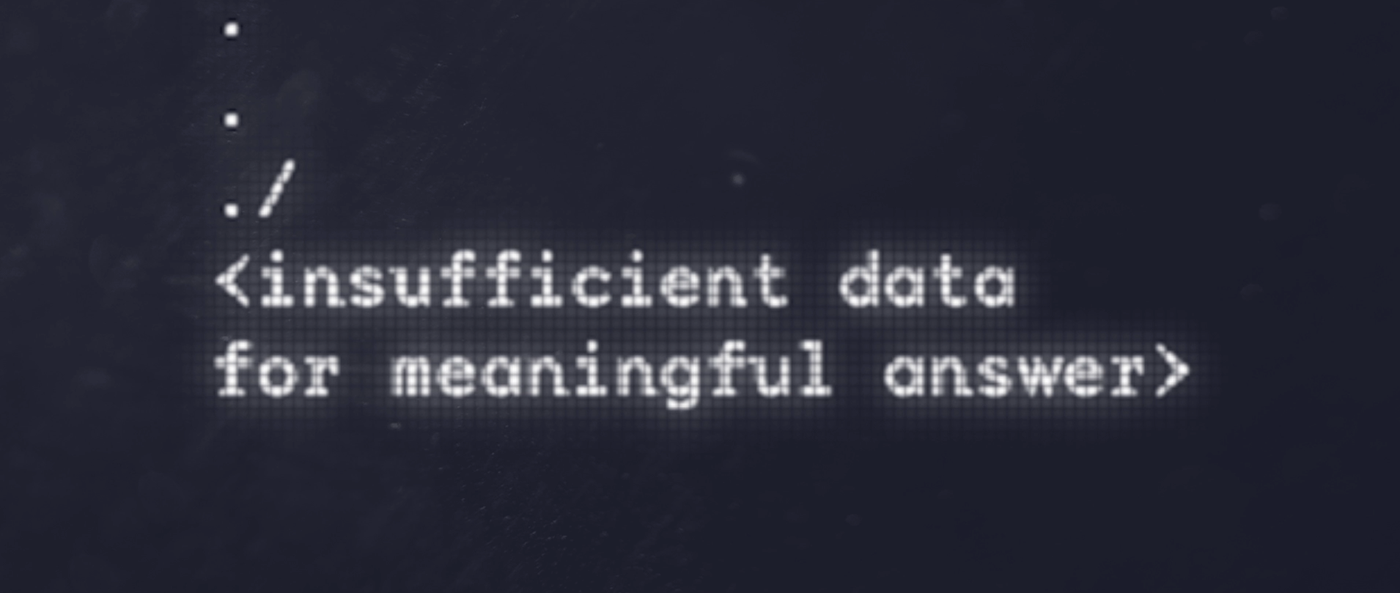
\includegraphics[width=60mm]{./lq}}
% %     \subfigure[Figure B]{\label{fig:b}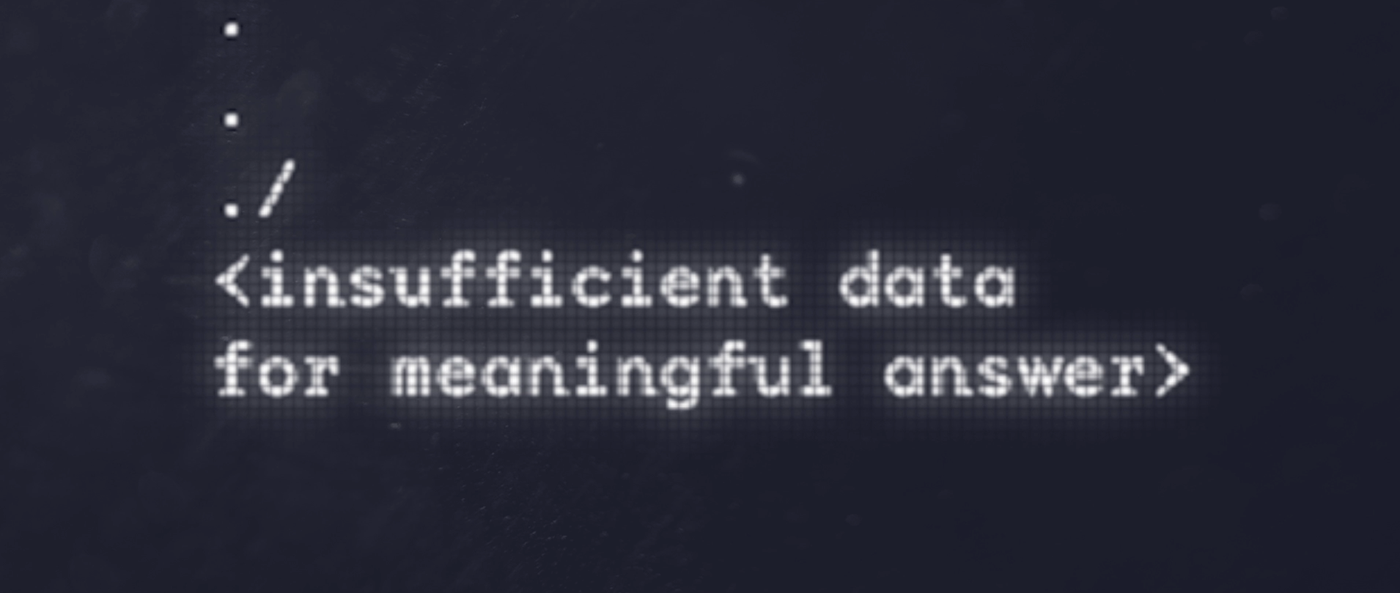
\includegraphics[width=60mm]{./lq}}
% %     \subfigure[Figure C]{\label{fig:c}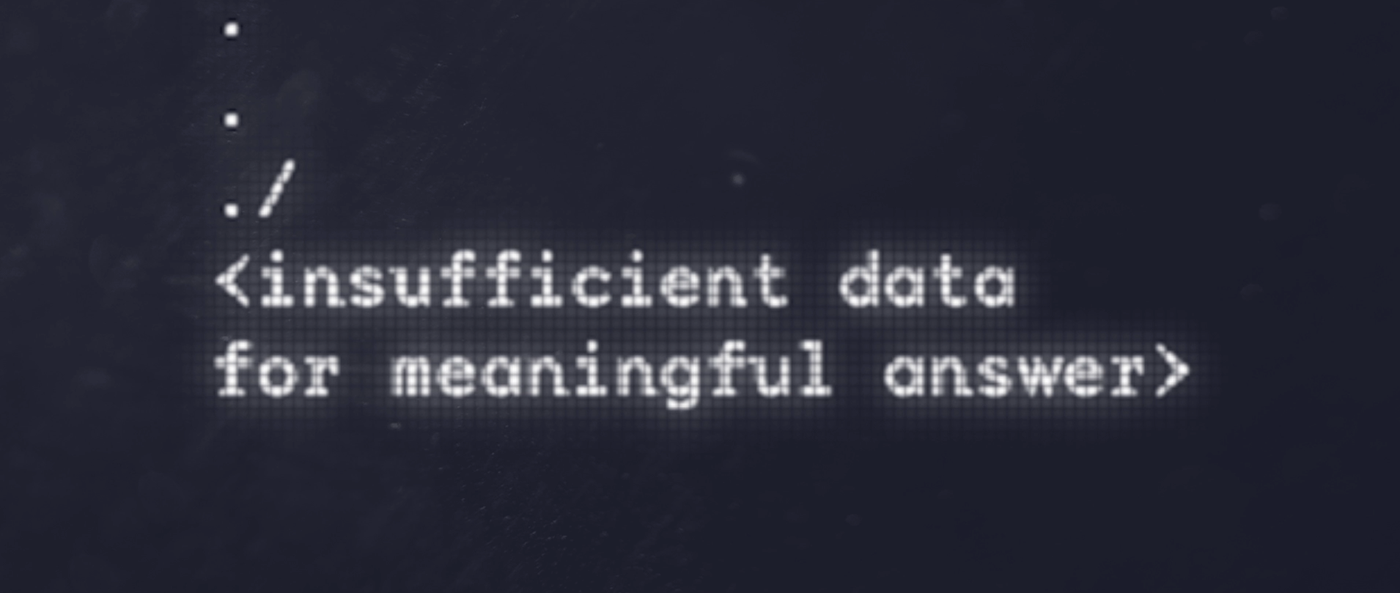
\includegraphics[width=\textwidth]{./lq}}
% %     \caption{Three simple graphs}
% %     \label{fig:three graphs}
% % \end{figure}
% %----------------------------------------------------------

% % \begin{figure}
% %     \centering
% %     \begin{subfigure}[b]{0.3\textwidth}
% %         \centering
% %         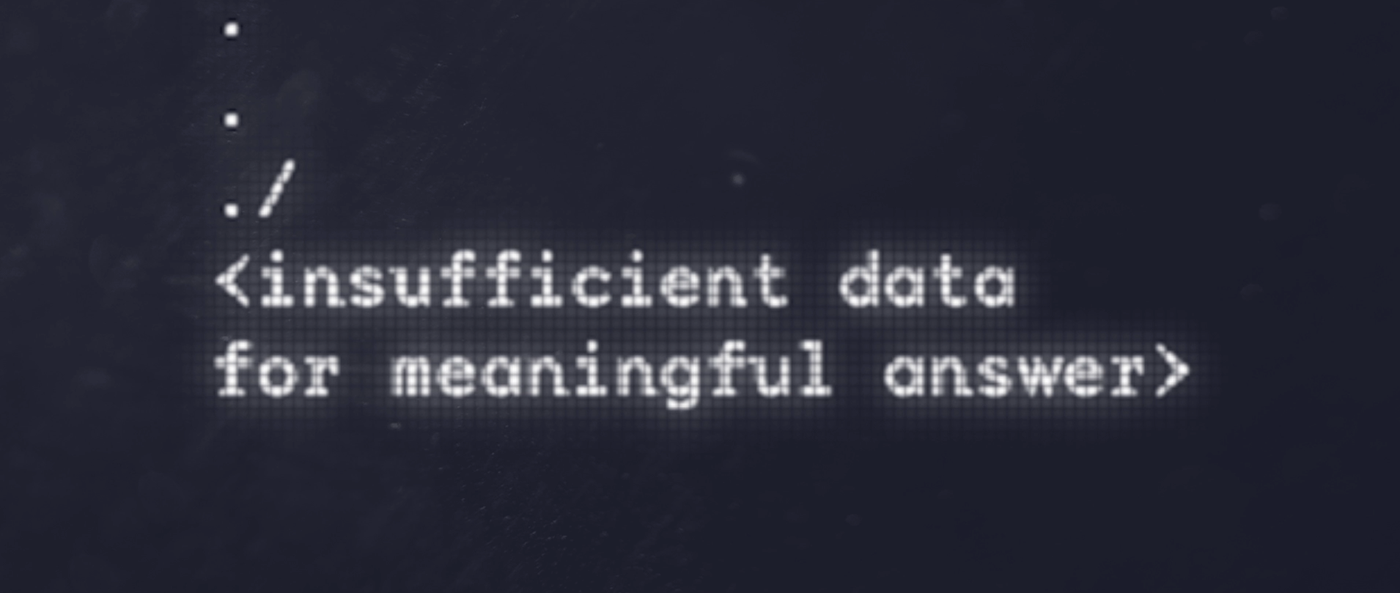
\includegraphics[width=\textwidth]{./lq}
% %         \caption{$y=x$}
% %         \label{fig:y equals x}
% %     \end{subfigure}
% %     \hfill
% %     \begin{subfigure}[b]{0.3\textwidth}
% %         \centering
% %         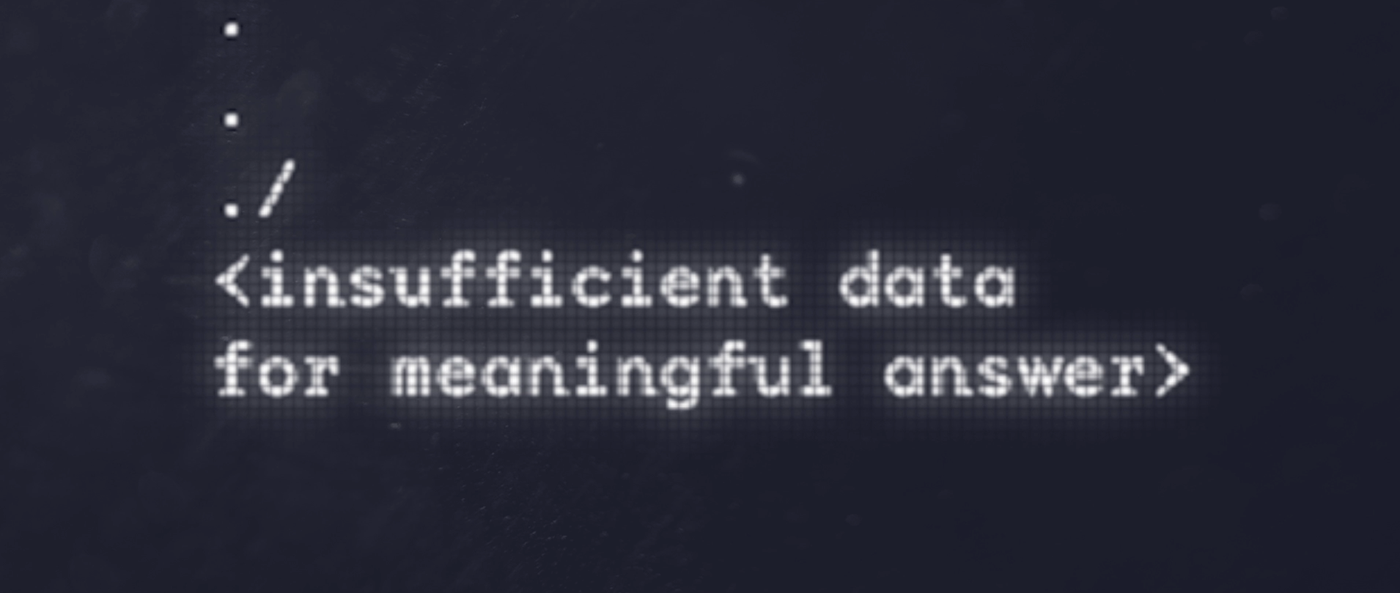
\includegraphics[width=\textwidth]{./lq}
% %         \caption{$y=3sinx$}
% %         \label{fig:three sin x}
% %     \end{subfigure}
% %     \hfill
% %     \begin{subfigure}[b]{0.3\textwidth}
% %         \centering
% %         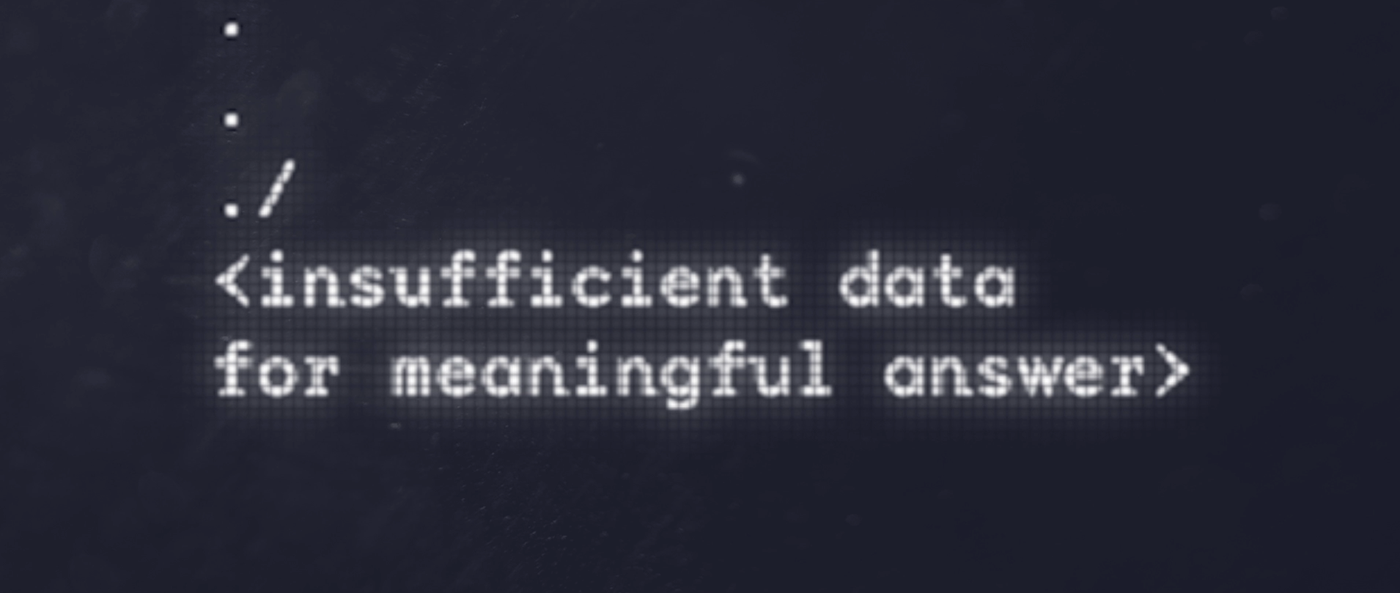
\includegraphics[width=\textwidth]{./lq}
% %         \caption{$y=5/x$}
% %         \label{fig:five over x}
% %     \end{subfigure}
% %        \caption{Three simple graphs}
% %        \label{fig:three graphs}
% % \end{figure}


% % %--------- NEW SECTION ----------------------
% % \section{Assunto 2}
% % \label{sec:ass2}
% % flkjasdlkfjasdlkfjs

% % \begin{table}[h]
% %     \begin{subtable}[h]{0.45\textwidth}
% %         \centering
% %         \begin{tabular}{l | l | l}
% %         Day & Max Temp & Min Temp \\
% %         \hline \hline
% %         Mon & 20 & 13\\
% %         Tue & 22 & 14\\
% %         Wed & 23 & 12\\
% %         Thurs & 25 & 13\\
% %         Fri & 18 & 7\\
% %         Sat & 15 & 13\\
% %         Sun & 20 & 13
% %        \end{tabular}
% %        \caption{First Week}
% %        \label{tab:week1}
% %     \end{subtable}
% %     \hfill
% %     \begin{subtable}[h]{0.45\textwidth}
% %         \centering
% %         \begin{tabular}{l | l | l}
% %         Day & Max Temp & Min Temp \\
% %         \hline \hline
% %         Mon & 17 & 11\\
% %         Tue & 16 & 10\\
% %         Wed & 14 & 8\\
% %         Thurs & 12 & 5\\
% %         Fri & 15 & 7\\
% %         Sat & 16 & 12\\
% %         Sun & 15 & 9
% %         \end{tabular}
% %         \caption{Second Week}
% %         \label{tab:week2}
% %      \end{subtable}
% %      \caption{Max and min temps recorded in the first two weeks of July}
% %      \label{tab:temps}
% % \end{table}
    \chapter{Desenvolvimento do projeto}
\label{chap:metod}
Este capítulo detalha o processo inicial de desenvolvimento do site de portfólio fotográfico, desde a concepção da ideia até a definição do design. Serão apresentados a ideação do projeto, as especificações técnicas e as funcionalidades implementadas.
\subsection{Metodologia do projeto}
A metodologia utilizada para o desenvolvimento deste projeto foi baseada no modelo \textit{Waterfall} (cascata), que é um modelo de desenvolvimento de software linear e sequencial. Este modelo é caracterizado por fases distintas, onde cada fase deve ser concluída antes do início da próxima. As fases do modelo \textit{Waterfall} incluem: requisitos, design, implementação, verificação e manutenção.

\section{Ideação}
Nesta seção será apresentada a fase de concepção inicial do projeto, incluindo o levantamento de necessidades do cliente, as referências visuais discutidas, os objetivos definidos para o site e as primeiras decisões relacionadas à estrutura e funcionalidades da plataforma. Serão abordados os encontros realizados com o cliente, os principais insumos obtidos a partir do workshop e como essas informações foram transformadas em requisitos e diretrizes para o design e desenvolvimento do site institucional.

%escrever oq sera apresentado

\subsection{Arquitetura Geral}
A arquitetura geral, apresentada na Figura \ref{fig:Arquitetura geral}, relaciona de modo geral a interface do usuário com a estrutura de apresentação do conteúdo e com os serviços externos integrados ao site. Neste contexto, a interface do usuário representa o ponto de acesso direto ao sistema por meio de navegadores em dispositivos móveis e desktops, permitindo a navegação entre páginas, visualização do portfólio e envio de mensagens de contato. A camada de serviços externos inclui integrações como formulários por e-mail (via Formspree) e redes sociais, como o Instagram.

 \begin{figure} [h!]	
    \centering

    \caption{Arquitetura Geral}
    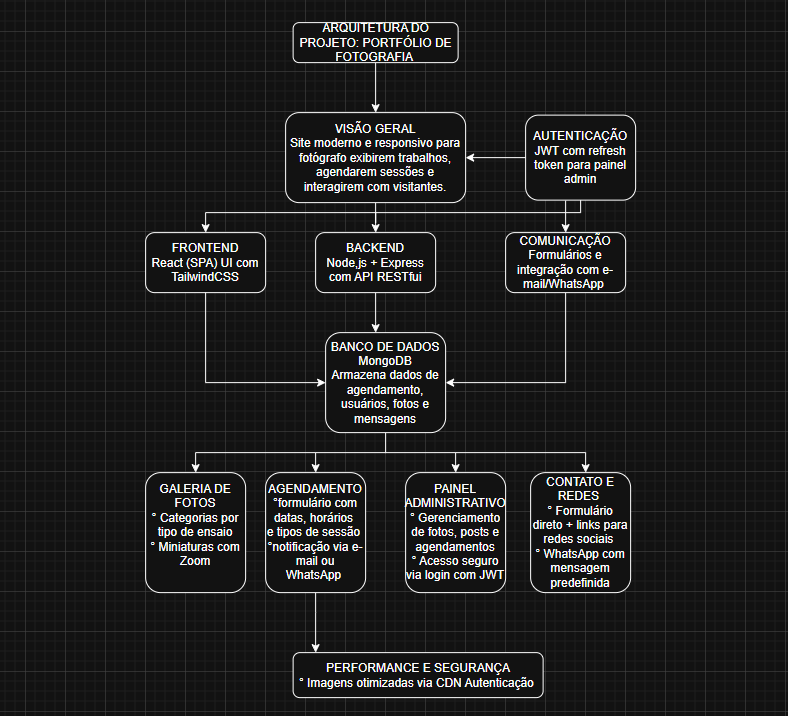
\includegraphics[width=0.9\textwidth]{Figures/Arquitetura_do_projeto.png}
    \caption*{Fonte: Autoria própria.}
    \label{fig:Arquitetura geral}
\end{figure}	

Para a estrutura de gerenciamento do site, utilizou-se um conjunto de tecnologias web padrão, incluindo HTML5, CSS3 e JavaScript no front-end. Essa camada é responsável por controlar as principais funcionalidades do sistema: exibição da galeria de fotos com filtros por categoria, navegação entre seções, exibição de informações institucionais, envio de mensagens por meio do formulário de contato e o sistema de agendamento de ensaios fotográficos. Este último permite que o usuário selecione uma data, horário e tipo de ensaio, com envio de confirmação por e-mail.

\subsection{Requisitos técnicos}
Os requisitos técnicos do site foram definidos com base nas demandas do cliente identificadas durante o workshop de levantamento de requisitos. A equipe utilizou uma abordagem inspirada no \textit{Quality Function Deployment} (QFD) para converter as necessidades funcionais e expectativas em características técnicas específicas que pudessem ser implementadas de forma objetiva e eficiente. Os principais requisitos definidos para o sistema foram:

\begin{itemize}
    \item O site deve ser 100\% responsivo, garantindo uma boa experiência em smartphones, tablets e desktops;
    \item As imagens devem ser otimizadas para carregamento rápido, com uso de técnicas como compressão e \textit{lazy loading};
    \item O layout deve seguir uma identidade visual alinhada à preferência do cliente (preto, branco e dourado), com foco em simplicidade e elegância;
    \item A galeria deve permitir filtragem por categorias (casamento, ensaio, corporativo, etc.);
    \item Deve ser possível realizar o agendamento de ensaios fotográficos com data, horário e tipo de serviço;
    \item O formulário de contato deve ser integrado ao e-mail do cliente e conter botão de WhatsApp;
    \item O sistema deve enviar confirmações de agendamento automaticamente por e-mail;
    \item O tempo médio de carregamento das páginas não deve ultrapassar 3 segundos;
    \item O código-fonte deve ser organizado, documentado e versionado com GitHub;
    \item O site deve permitir manutenção e expansão futura, como adição de blog ou painel administrativo.
\end{itemize}
%desdobramento da função qualidade
% \subsection{Quality Function Deployment}
% \textit{Quality Function Deployment} é uma ferramenta de qualidade que auxilia na conversão das demandas do cliente em características de qualidade do produto. Dessa forma, no primeiro ciclo do QFD foram analisados os requisistos do cliente e os requisitos técnicos necessários, sinalizando os pontos mais importantes e as relações entre estes. O resultado foi exposto na \ref{fig:QFD}

% \begin{figure} [h!]	
%     \centering
%     \caption{ Primeiro ciclo QFD}
%     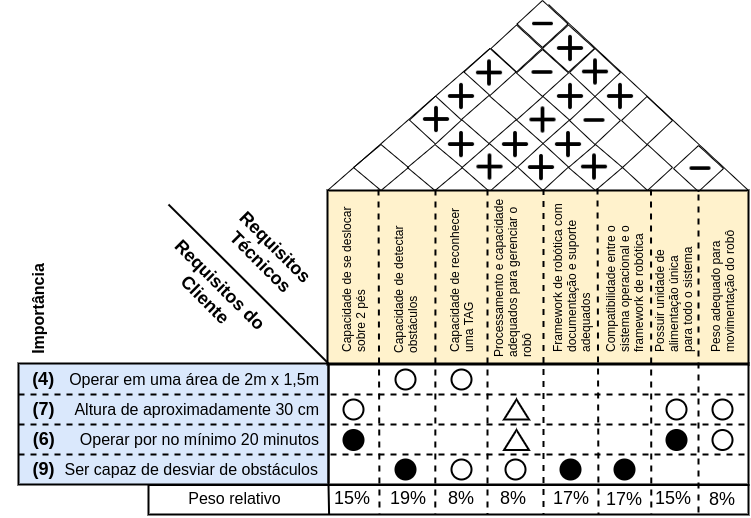
\includegraphics[width=0.8\textwidth]{Figures/QFD}
%     \caption*{Fonte: Autoria própria.}
%     \label{fig:QFD}
% \end{figure}
%  Através do QFD foi possível observar 

% % %--------- NEW SECTION ----------------------
% % \section{Interface do Usuário}
% % \label{sec:ui}
% % \lipsum[1]

% % %--------- NEW SECTION ----------------------
% % \section{Simulação do sistema}
% % \label{sec:sim}
% % \lipsum[2-4]
\subsection{Modelagem dos processos}

\begin{figure} [h!]	
    \centering

    \caption{Modelo esquemático dos processos}
    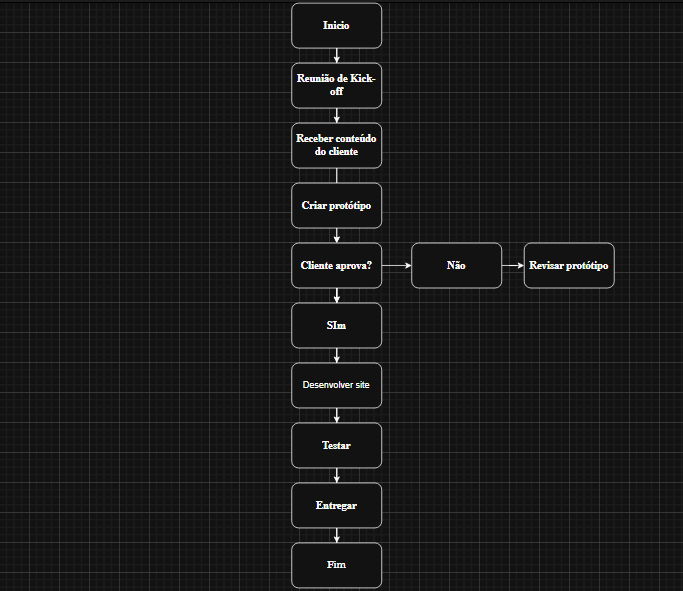
\includegraphics[width=0.9\textwidth]{Figures/modelo_esquematico_dos_processos.png}
    \caption*{Fonte: Autoria própria.}
    \label{fig:modelagem_dos_processos}
\end{figure}

    \chapter{Resultados}
\label{chap:result}
Importante sempre ter um parágrafo introdutório para explicar os resultados encontrados.

% %--------- NEW SECTION ----------------------
% \section{Testes unitários}
% \label{sec:testu}
% \lipsum[1]

% \section{Integração do sistema}
% \label{sec:intsis}
% \lipsum[1]

% %--------- NEW SECTION ----------------------
% \section{Testes integrados}
% \label{sec:testi}
% \lipsum[1]

\section{Diagrama de classes}
\label{sec:class}
O diagrama de classes é uma representação visual das classes do sistema e seus relacionamentos. Ele é utilizado para descrever a estrutura do sistema e como as classes interagem entre si. A Figura \ref{fig:diagrama_classes} apresenta o diagrama de classes do sistema desenvolvido.
\begin{figure} [h!]	
    \centering
    \caption{Meu diagrama de classes}
    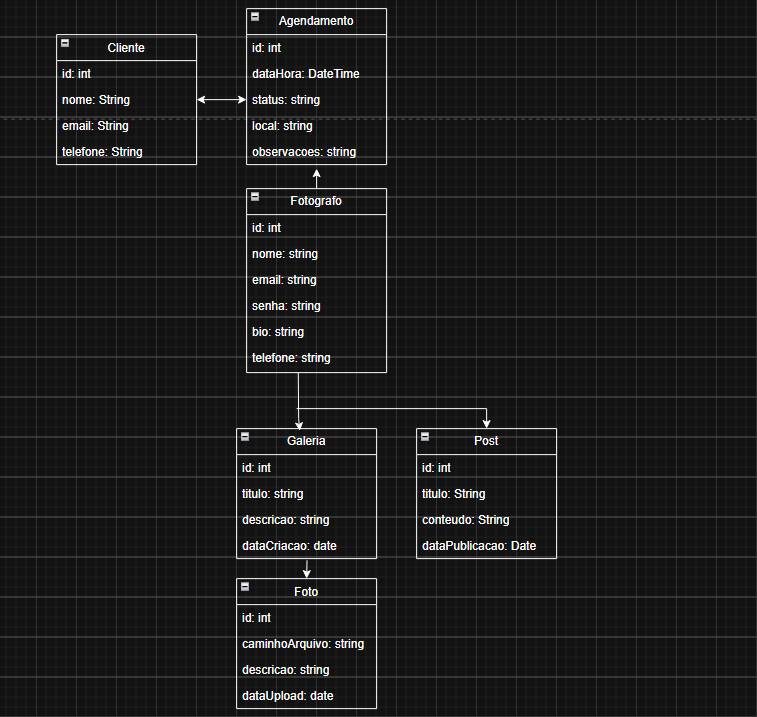
\includegraphics[width=0.9\textwidth]{Figures/Diagrama_de_Classes.png}
    \caption*{Fonte: Autoria própria.}
    \label{fig:diagrama_classes}
\end{figure}

favor olhar a seção \ref{sec:class}.


\section{Diagrama de casos de uso}
\label{sec:casos}
O diagrama de casos de uso é uma representação visual dos casos de uso do sistema e os atores envolvidos. Ele é utilizado para descrever as funcionalidades do sistema e como os usuários interagem com ele. A Figura \ref{fig:diagrama_casos} apresenta o diagrama de casos de uso do sistema desenvolvido.
\begin{figure} [h!]
    \centering
    \caption{Meu diagrama de casos de uso}
    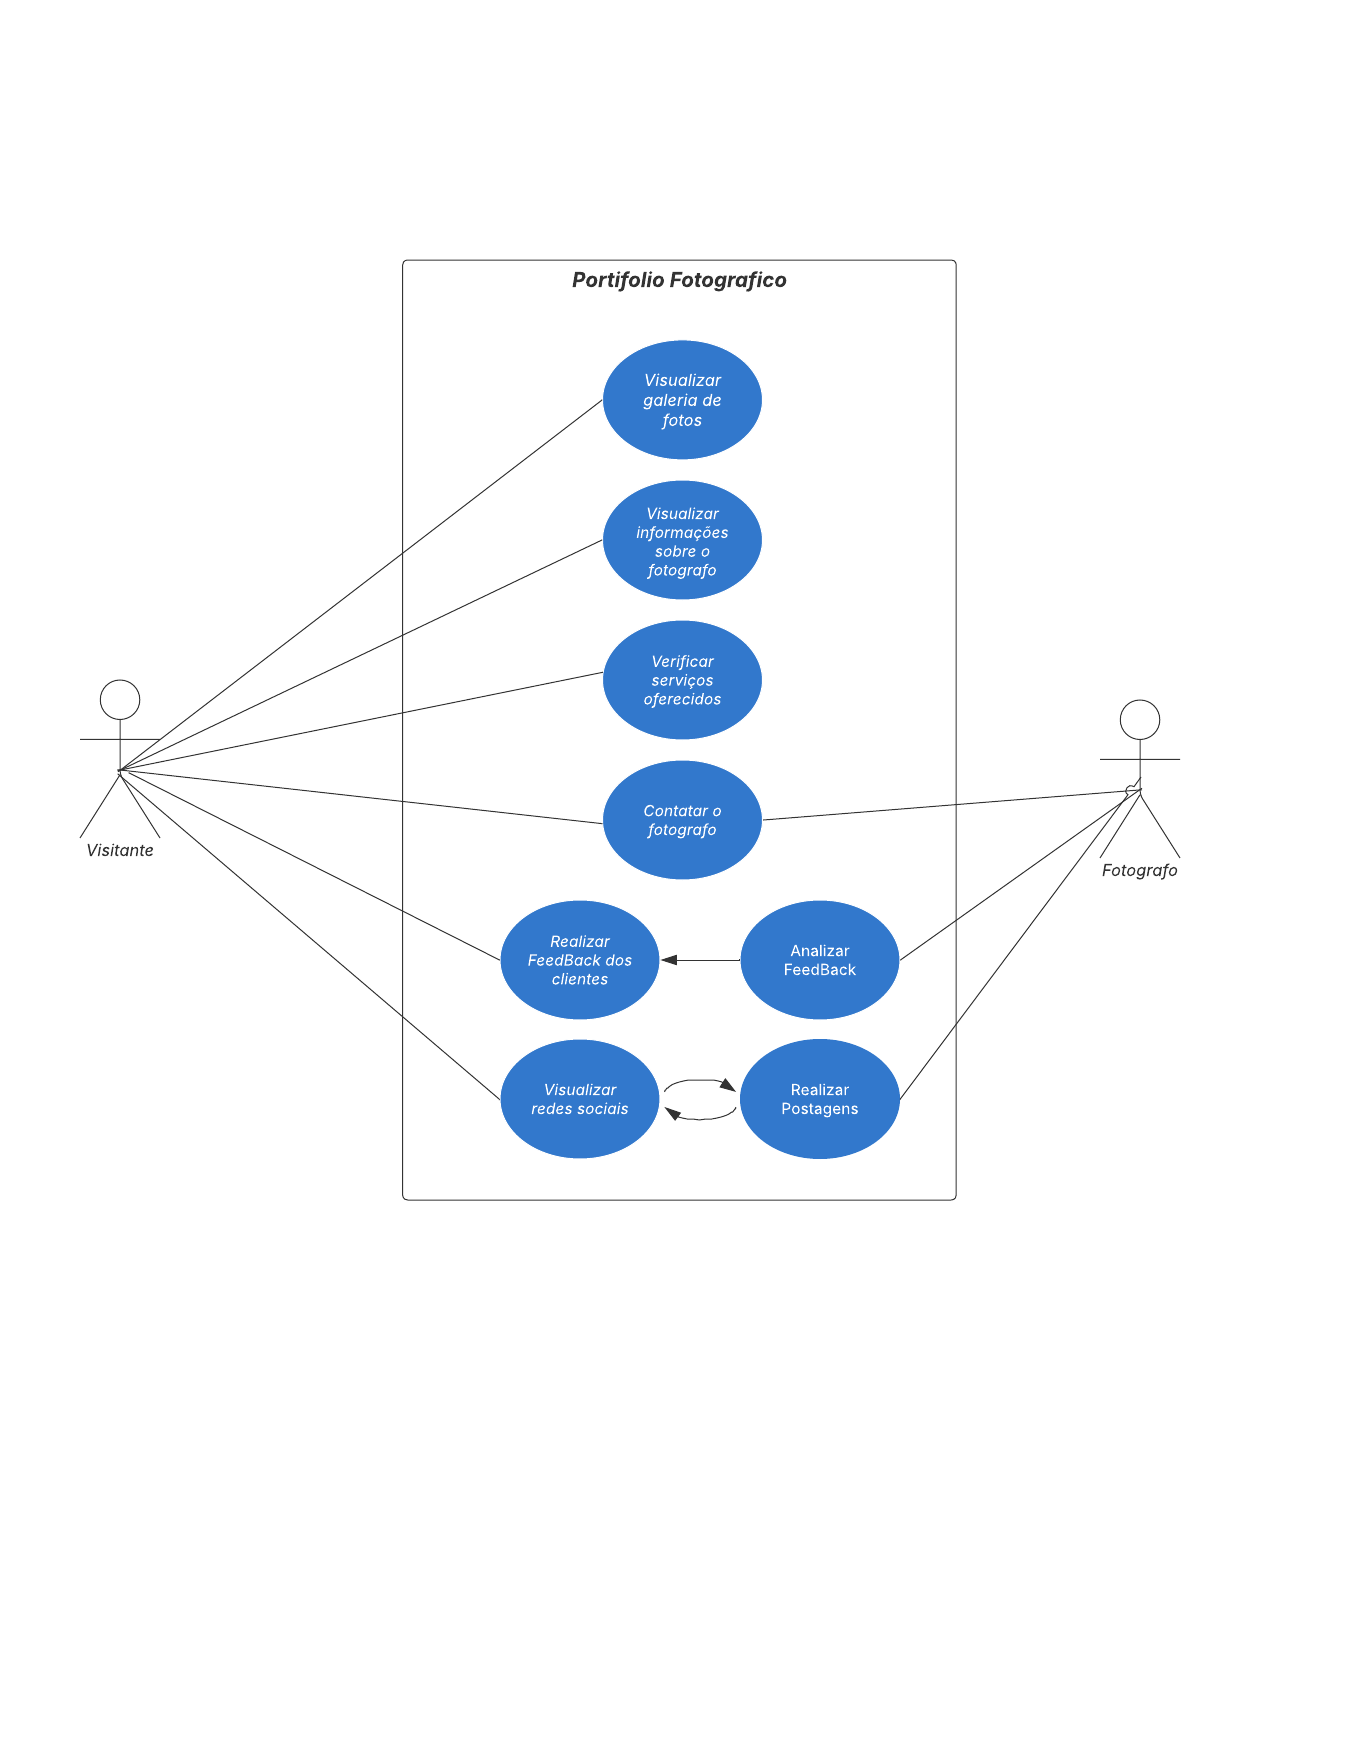
\includegraphics[width=0.9\textwidth]{Figures/Diagrama_de_caso_de_uso.png}
    \caption*{Fonte: Autoria própria.}
    \label{fig:diagrama_de_casos_de_uso}
\end{figure}

\section{Diagrama de sequência}
\label{sec:sequencia}   
O diagrama de sequência é uma representação visual da interação entre os objetos do sistema ao longo do tempo. Ele é utilizado para descrever como os objetos interagem entre si para realizar uma determinada funcionalidade. A Figura \ref{fig:diagrama_sequencia} apresenta o diagrama de sequência do sistema desenvolvido. 
\begin{figure} [h!]	
    \centering
    \caption{Meu diagrama de sequência}
    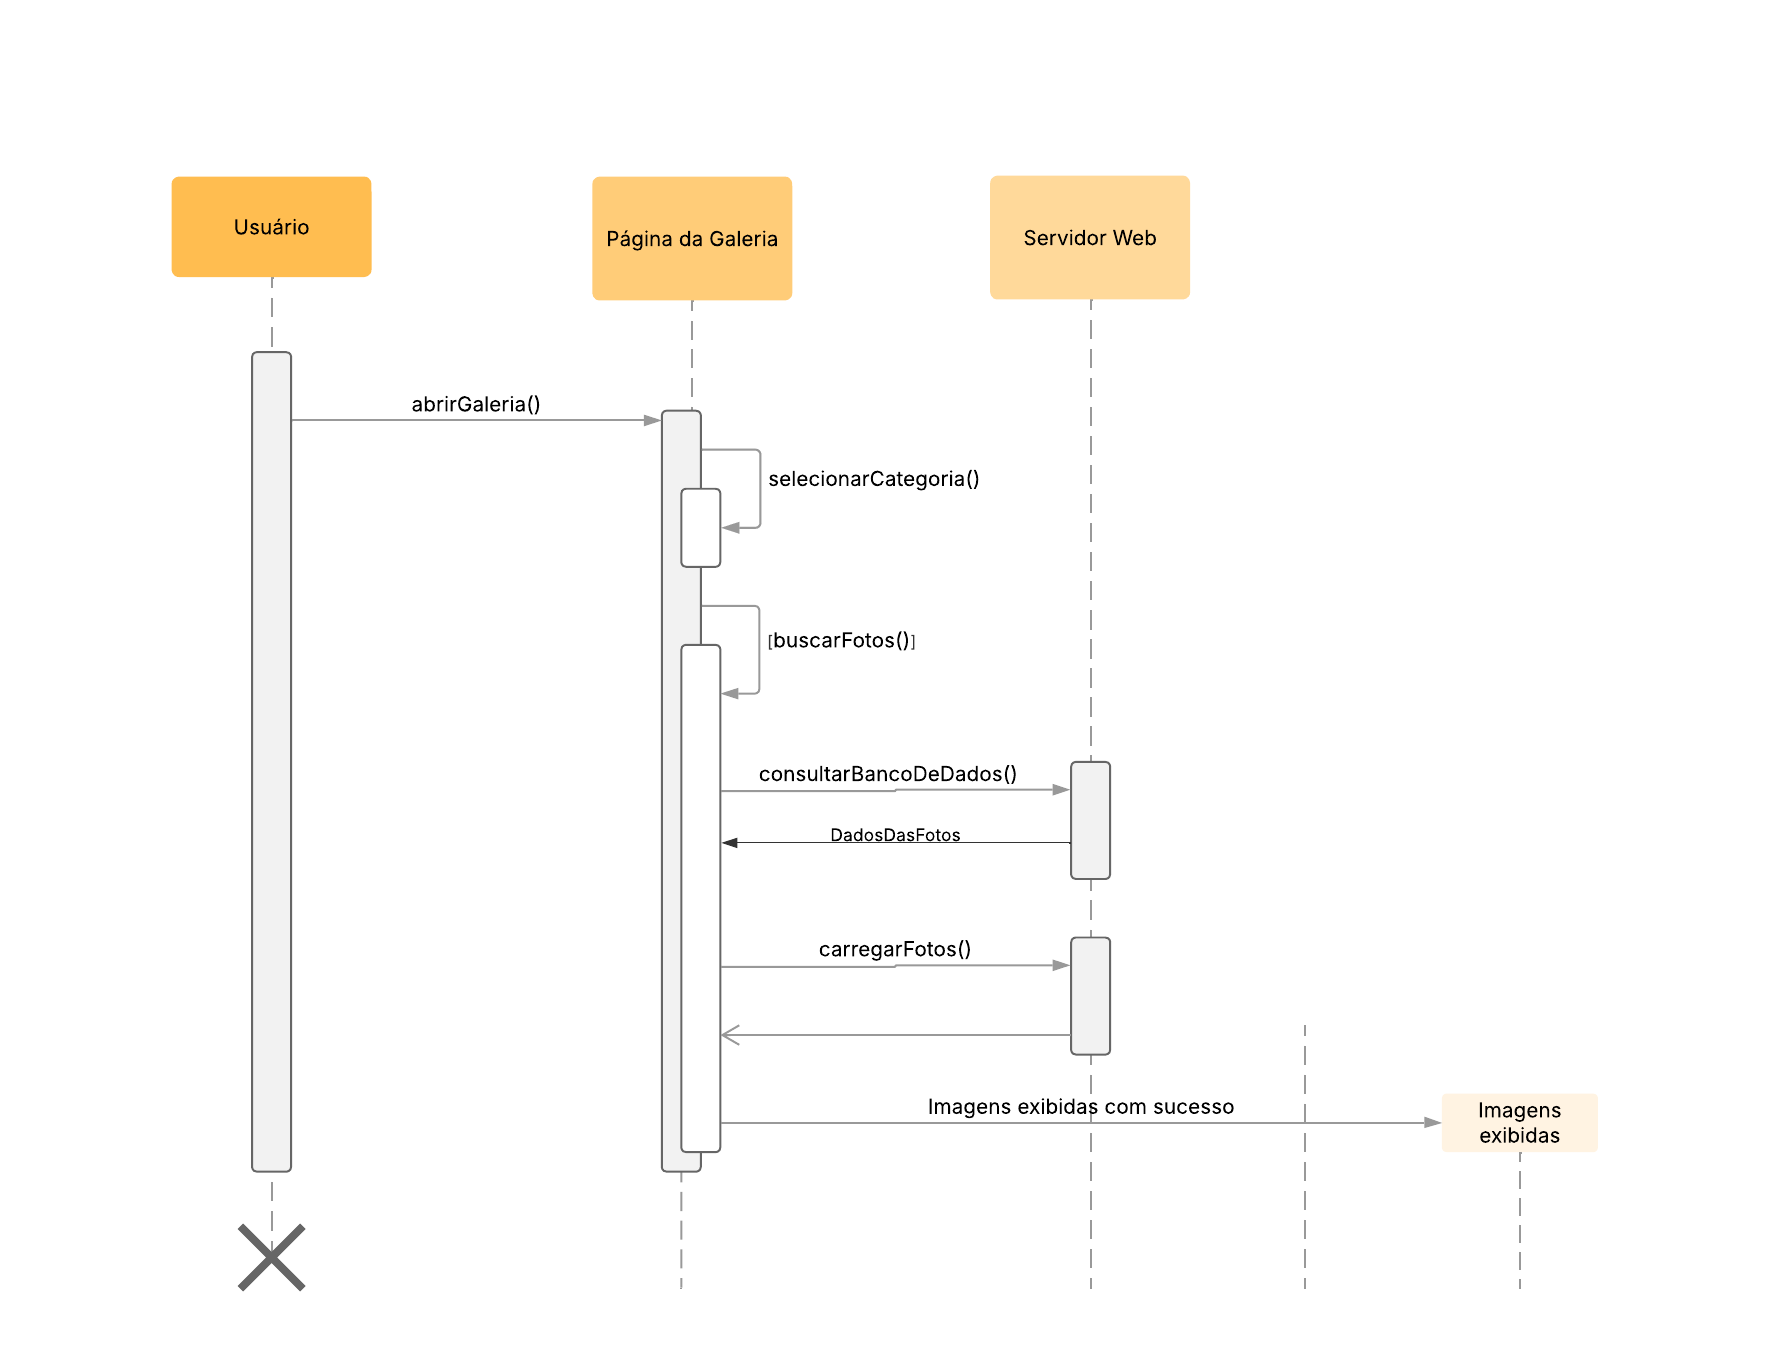
\includegraphics[width=0.9\textwidth]{Figures/Diagrama_de_sequência_básico.png}
    \caption*{Fonte: Autoria própria.}
    \label{fig:diagrama_de_sequencia}
\end{figure}








    \chapter{Conclusão}
\label{chap:conc}

O desenvolvimento do site institucional para o fotógrafo Geovany demonstrou a viabilidade de criar uma plataforma leve, responsiva e de fácil manutenção, alinhada às necessidades de divulgação de portfólio e captação de clientes. Ao longo das etapas do modelo Waterfall — levantamento de requisitos, prototipação, implementação, testes e entrega — foi possível mapear com clareza as demandas do cliente e traduzi-las em funcionalidades concretas: galeria filtrável por categorias, sistema de agendamento de ensaios, formulário de contato integrado ao e-mail e WhatsApp, além de integrações com Instagram e meios de pagamento.

A adoção de boas práticas de UX/UI e otimização de performance (compressão de imagens e lazy loading) garantiu um tempo médio de carregamento abaixo de 3 segundos, conforme previsto nos requisitos técnicos. A prototipação no Figma e o uso de Kanban no Trello facilitaram a comunicação entre a equipe e a obtenção de feedbacks rápidos do cliente, resultando em um produto final que atende plenamente ao escopo definido.



\section{Considerações finais}
\label{sec:consid}

A experiência proporcionada por este projeto reforça a importância de um processo de desenvolvimento estruturado e centrado no usuário. Do ponto de vista acadêmico, o trabalho permitiu aplicar conceitos de gestão de projetos, modelagem de requisitos e desenvolvimento web em um caso real, promovendo o aprendizado colaborativo e prático.  

Tecnicamente, a entrega de um site responsivo com funcionalidades completas — incluindo agendamento online e integração com serviços externos — agrega valor ao fotógrafo, ampliando sua visibilidade digital e potencial de negócios. Socialmente, contribui para a profissionalização de pequenos empreendedores criativos, que dependem cada vez mais de soluções digitais acessíveis.

Em termos de perspectivas futuras, recomenda-se explorar a inclusão de um painel administrativo mais robusto, análise de métricas de uso (via Google Analytics) e evolução para uma versão multilíngue. Essas melhorias podem ampliar o alcance do site e oferecer insights valiosos para o cliente sobre o comportamento dos visitantes.











    % include more chapters ...
%
% ----------------------------------------------------------------------------
% Include thesis appendices
    \begin{thesisappendices}
        \include{Appendices/diagmec}
        \include{Appendices/diagele}
        %\include{Appendices/logbook}
    \end{thesisappendices}
%
% ----------------------------------------------------------------------------
% Configurar as referencias bibliograficas
  	\renewcommand\bibname{Referências}
    \addcontentsline{toc}{chapter}{Referências}
    \bibliography{References/referencias}
%
% ----------------------------------------------------------------------------
% Finishing him
    \include{Others/ultimafolha}
\end{document}
%
% -------------------------------------------------------------------------------
% Aqui termina a formatação para o documento.
% In God We Trust. All Other Bring Data. 
%
% -------------------------------------------------------------------------------